%!TEX root = chapter-methodology.tex
\section{Region of Interest Extraction}
\label{sec:methodology:roiextraction}

The raw 3D palmprint image consists of 768*576 pixels with a depth value at each point. The samples are captured by a 3D palmprint acquisition device based on structured light imaging ~\cite{Zhang:2009dp}. Before any other processing, noisy pixels at the boundaries must be removed. The full resolution sample is cropped to a Region of Interest (ROI) with 400*400 resolution. A rectangle mask, from (234,68) to (634,468) is used to crop the ROI. Figure ~\ref{fig:methodology:sample-fullres} shows a full resolution sample of a palmprint and Figure ~\ref{fig:methodology:sample-roi} shows the ROI cropped. To reduce the storage and computation requirements for further processing, the ROI is down-sampled to a resolution of 200*200.

\begin{figure}[htb]
\begin{center}
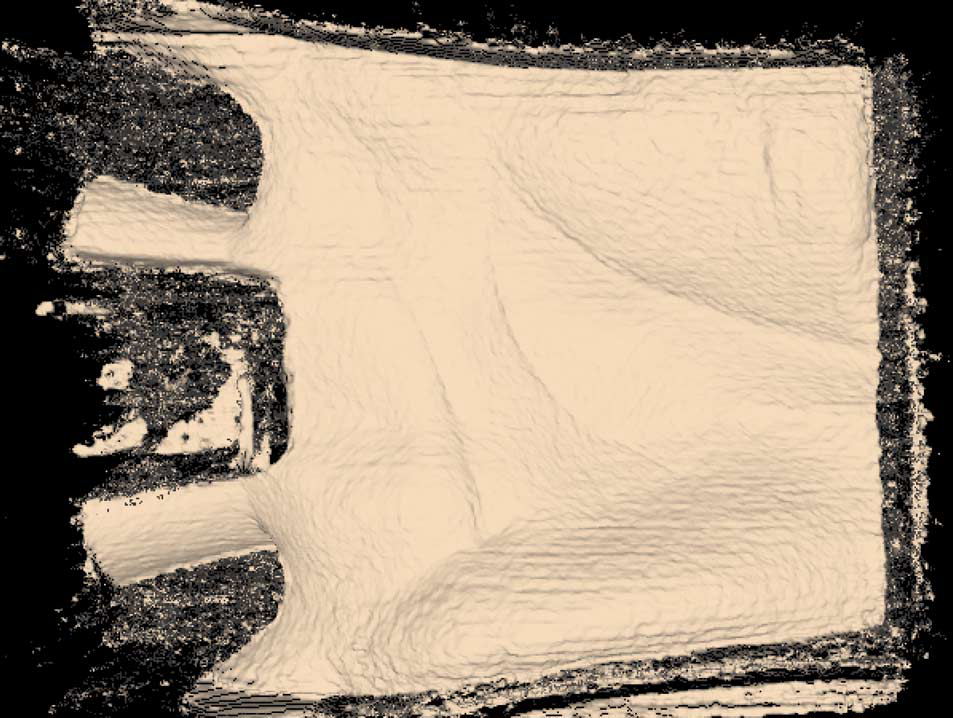
\includegraphics[width=0.9\linewidth]{ch-methodology/figures/sample-fullres}
\caption[Full resolution 3-D palmprint sample]{Full resolution 3-D palmprint sample}    \label{fig:methodology:sample-fullres}
\end{center}
\end{figure}

\begin{figure}[htb]
\begin{center}
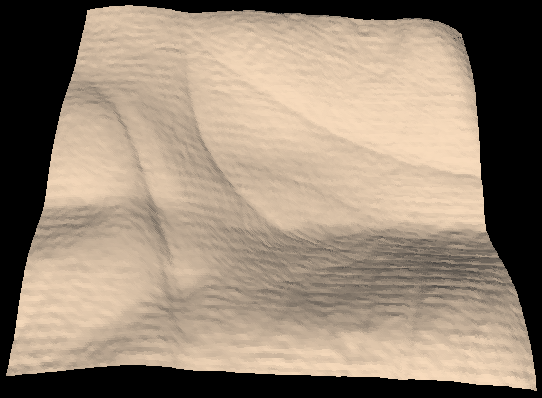
\includegraphics[width=0.9\linewidth]{ch-methodology/figures/sample-roi}
\caption[ROI from a 3-D palmprint sample]{ROI from a 3-D palmprint sample}
\label{fig:methodology:sample-roi}
\end{center}
\end{figure}

The ROI data is stored in a 200 by 200 matrix,

\begin{equation}
\label{eq:methodology:roimatrix}
D=d_{ij}|i=1,2,\dots,200; j=1,2,\dots,200
\end{equation}

where $d_{ij}$ is the depth value of the $i^{th}$ row and $j^{th}$ column pixel of the ROI.

%TODO find the citation
There exists more complicated ROI extraction methods taking advantage of the 2D approaches. 2D ROI is first obtained using the algorithm in ~\cite{Zhang:2003uf}. As the 2D sample captured is pixel-to-pixel matched to the 3D sample, using the exact 2D ROI for the 3D sample is trivial.

The cropping ROI extraction approach used here is much easier and faster than the one proposed in [4]. The reason to adopt this naive approach is that the features are invariant to rotation and translation. It is unnecessary to fully align every sample. Another consideration is that when the 3D information is the only data available, it is not feasible to apply the same 2D algorithm to the depth image.

Even if the samples are cropped to the center area, it is still possible that some noisy pixels are included. If the gradient

\begin{equation}
|\nabla D|=\sqrt{
\left(\frac{\partial{D}}{\partial{x}}\right)^2 +
\left(\frac{\partial{D}}{\partial{y}}\right)^2
}
\end{equation}

is larger than a given threshold, the pixel is regarded as noisy. Another 200 by 200 matrix,

\begin{equation}
\label{eq:methodology:roimask}
M=m_{ij}|i=1,2,\dots,200;j=1,2,\dots,200
\end{equation}

is used to represent the mask, where $m_{ij}=0$ marks the noisy pixels while $m_{ij}=1$ marks the normal ones.